\textbf{Wersja podstawowa modelu ze zmienną liczbą wierzchołków i walidacją krzyżową}

Model uczony na grafach ze zmienną liczbą wierzchołków oraz zastosowaną walidacją krzyżową,
bardzo szybko osiąga poziom dokładności biski 100\%, bo już w kilku pierwszych epokach.
Po około 10 epoce, dokonuje się stabilizacja, oscylująca między 95\%, a 100\%.
W przypadku tego modelu, fluktuacje dokładności są znikome, co wskazuje na dobrą stabilność modelu.
Pojedyncze przypadku spadu dokładności, mogą być spowodowane bardziej skomplikowanymi
przypadkami w zbiorze danych walidacyjnych.

Strata tego modelu gwałtownie spada na początku procesu uczenia,
po czym stabilizuje się na zadowalająco niskim poziomie - poniżej 20\%.
Skoki wskaźnika są bardziej zauważalne na zbiorze walidacyjnym,
ale nie wydają się być regularne i nie wpływają na ogólny wynik.
Mogą być wynikiem, przeuczenia na pojedynczych epokach lub naturalną zmiennością walidacyjnego zbioru danych.

\begin{figure}[ht]
	\centering
	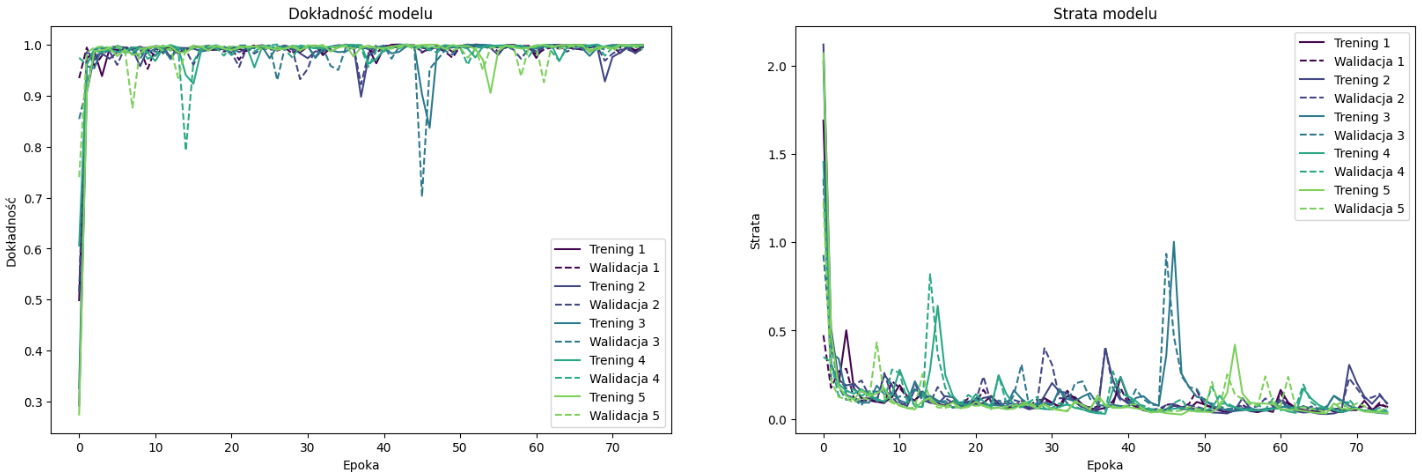
\includegraphics[height=5.5cm]{resources/tests/images/v3/multiple_edges_crossvalid_img.png}
	\caption{Dokładność i walidacja dla modelu ze zmienną liczbą wierzchołków i walidacją krzyżową}
	\label{Fig:tests-csvar-0a}
\end{figure}
\FloatBarrier

Model wydaje się dokładny na zbiorze treningowym i walidacyjnym,
co może skutkować polepszoną skutecznością w klasyfikacji grafów.
Minimalne różnice pomiędzy dokładnością treningową a walidacyjną wskazują na dobrą zdolność generalizacji.
Z otrzymanych wyników, wydawałoby się, że model nie uległ przeuczeniu,
choć jest to również możliwe, zważając na bardzo wysokie wyniki dokładności. 

\begin{figure}[ht]
	\centering
	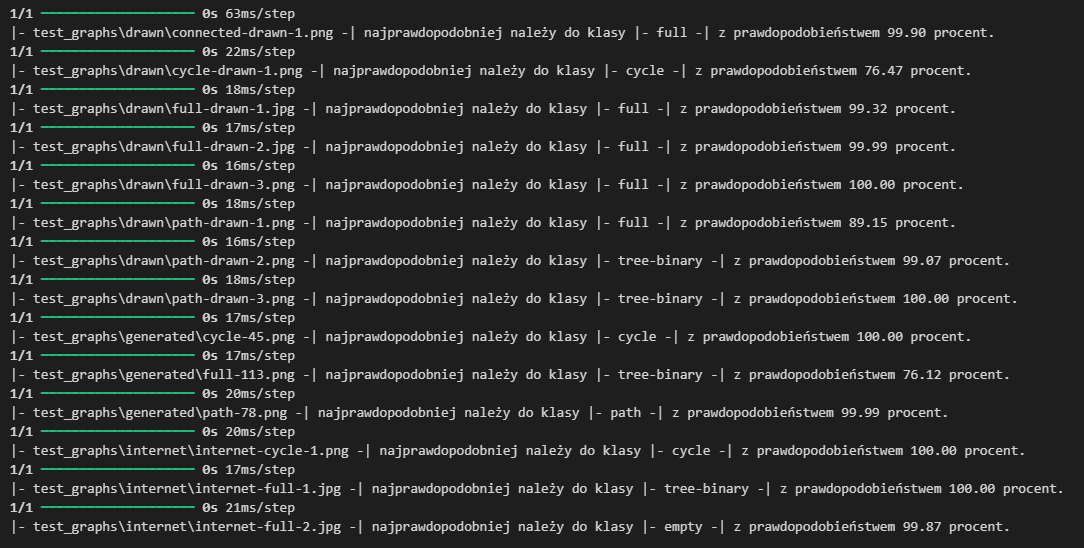
\includegraphics[height=5.5cm]{resources/tests/images/v3/multiple_edges_crossvalid_txt.png}
	\caption{Klasyfikacja obrazów zewnętrznych dla modelu ze zmienną liczbą wierzchołków i walidacją krzyżową}
	\label{Fig:tests-csvar-0b}
\end{figure}
\FloatBarrier

\begin{figure}[ht]
	\centering
	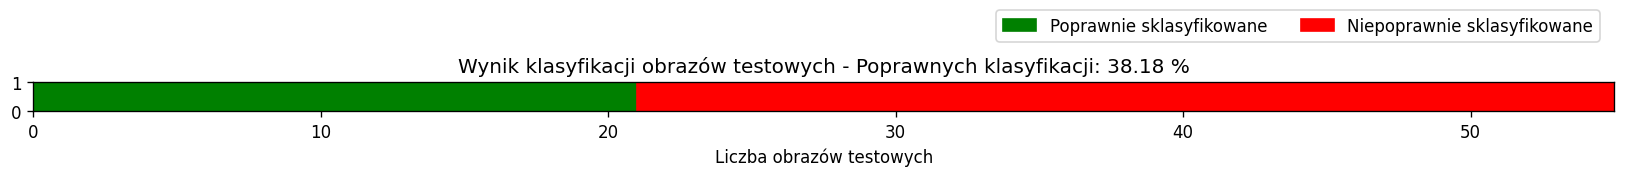
\includegraphics[width=14cm]{resources/tests/images/v3/multiple_edges_crossvalid_bar.png}
	\caption{Wizualizacja klasyfikacji obrazów zewnętrznych dla modelu ze zmienną liczbą wierzchołków i walidacją krzyżową}
	\label{Fig:tests-csvar-0c}
\end{figure}
\FloatBarrier

Model poprawnie sklasyfikował aż 38\% testowanych danych zewnętrznych.
Jest to zadowalający wynik, zważając na trudności innych modeli w poprawnym wskazywaniu klas sprawdzanych grafów.
Podejrzenia dotyczące przeuczenia modelu były więc bezpodstawne.
Model całkiem dobrze nauczył się żądanych wzorców.

\textbf{Zmodyfikowany model ze zmienną liczbą wierzchołków i walidacją krzyżową - Conv2D i Dropout oraz spowolnienie uczenia}

Model stosuje zwiększone parametry filtrów dla warstw Conv2D, powiększony parametr Dropout z 0,2 do 0,5
oraz spowolnienie uczenia.

Dokładność osiąga poziom bliski 100\% na zbiorze treningowym i walidacyjnym w bardzo szybkim tempie.
Po osiągnięciu tego pułapu, utrzymuje się na nim do ostatniej epoki procesu nauczania modelu.
Jedyną anomalię można zaobserować około 55 epoki dla jednego z przejść walidacji krzyżowej.
Spada ona gwałtownie do poziomu 23\% i pozostaje w takim stanie do końca nauki.

Strata prezentuje się podobnie jak dokładność.
Wartości utrzymują się na dość niskich poziomach przez cały proces uczenia po początkowym spadku.
Około 55 epoki, dla jednego przejścia walidacji krzyżowej,
da się zaobserować nagły wzrost straty do około 2,5 jednostek, który stopniowo spada do około 1,8.

\begin{figure}[ht]
	\centering
	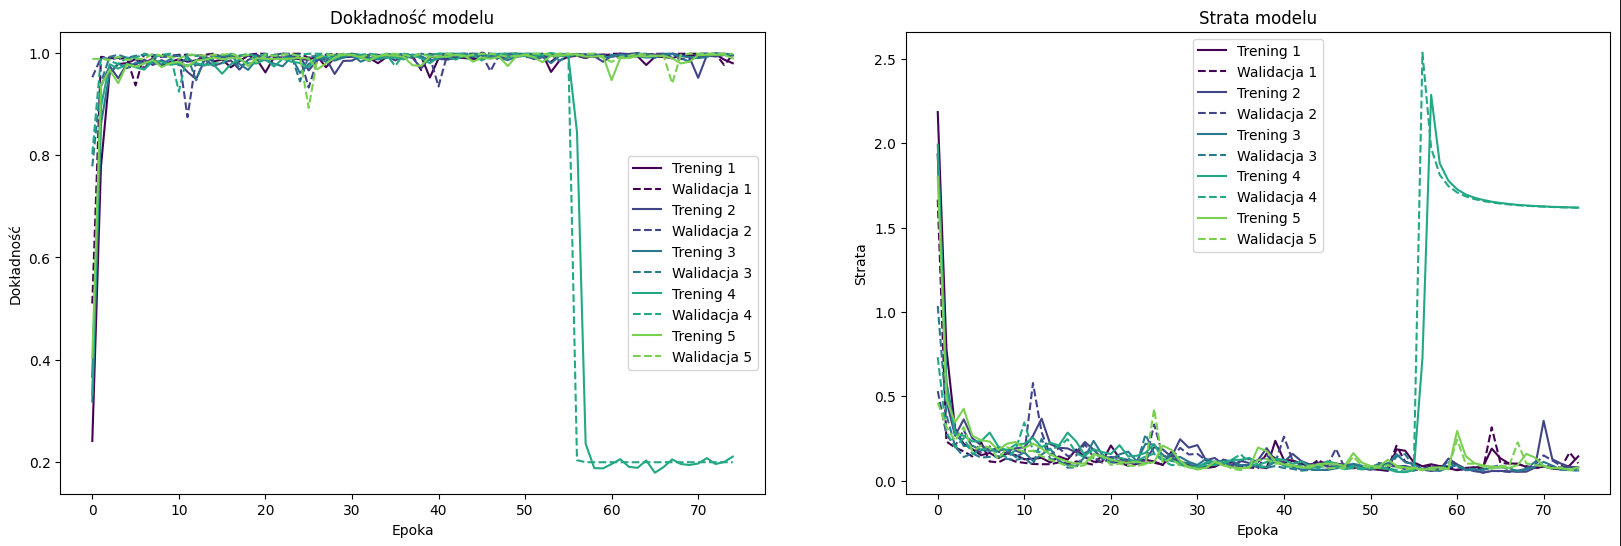
\includegraphics[height=5cm]{resources/tests/images/v4/multiple_edges_crossvalid_1_img.png}
	\caption{Dokładność i walidacja dla zmodyfikowanego modelu ze zmienną liczbą wierzchołków i walidacją krzyżową - Conv2D i Droput}
	\label{Fig:tests-csvar-1a}
\end{figure}
\FloatBarrier

W przypadku pojedynczej anomalii jaką da się zaobserować na krzywych dokładności oraz straty,
można wnioskować, że dla jednego przejścia walidacji krzyżowej, a konkretnie czwartego, wystąpił pewien problem z uczeniem modelu.
Mogła to być zmiana wartości współczynnika uczenia się lub inna zmiana w procesie treningu.
Różnice pomiędzy wartościami dla danych treningowych oraz waldacyjnych są znikome - nawet w przypadku odstającym wartościami od reszty.
Ogólnie, model osiągnął bardzo dobre wyniki, co sugeruje, że proces nauczania przebiegł pomyślnie.

\begin{figure}[ht]
	\centering
	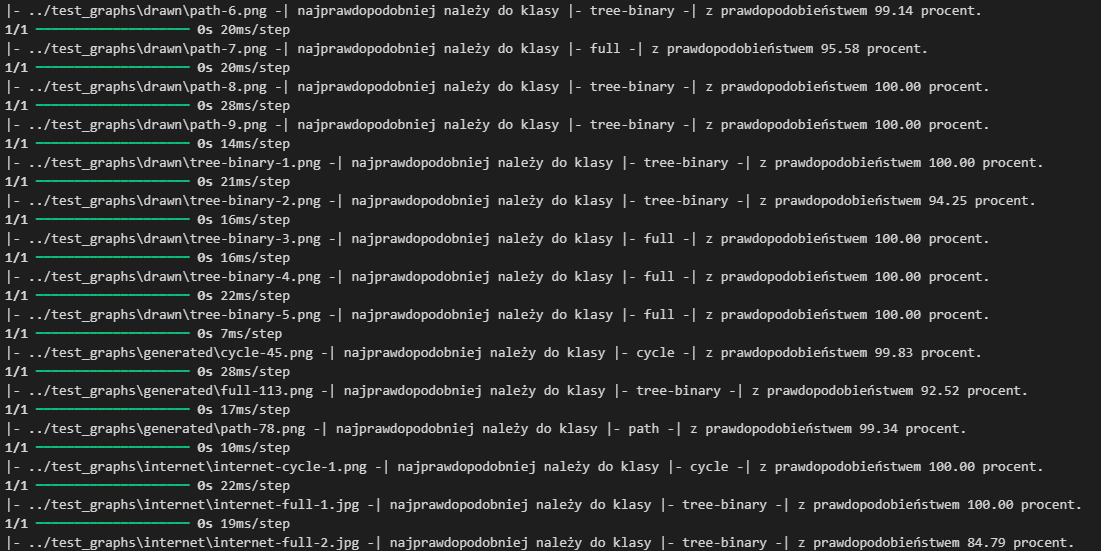
\includegraphics[width=14cm]{resources/tests/images/v4/multiple_edges_crossvalid_1_txt.png}
	\caption{Klasyfikacja obrazów zewnętrznych dla zmodyfikowanego modelu ze zmienną liczbą wierzchołków i walidacją krzyżową - Conv2D i Droput}
	\label{Fig:tests-csvar-1b}
\end{figure}
\FloatBarrier

\begin{figure}[ht]
	\centering
	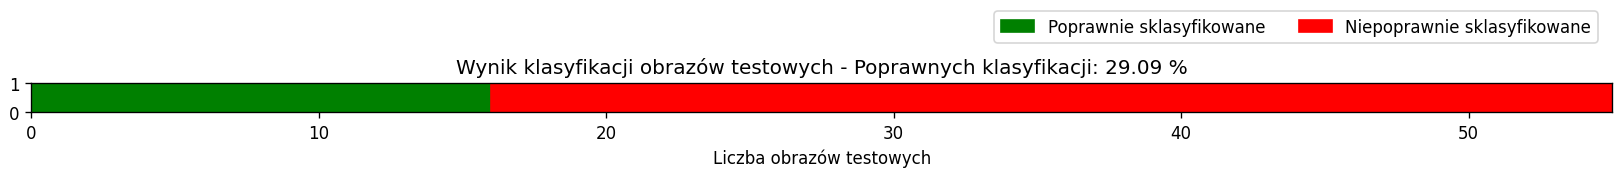
\includegraphics[width=14cm]{resources/tests/images/v4/multiple_edges_crossvalid_1_bar.png}
	\caption{Wizualizacja klasyfikacji obrazów zewnętrznych dla zmodyfikowanego modelu ze zmienną liczbą wierzchołków i walidacją krzyżową - Conv2D i Droput}
	\label{Fig:tests-csvar-1c}
\end{figure}
\FloatBarrier

Poprawna klasyfikacja 29\% grafów jest w pewnym sensie rozczarowującym wynikiem,
zważajac na wysokie wartości dokładności, nawet na zbiorach walidacyjnych
oraz całkiem wysoki wynik modelu bez modyfikacji.
Wnioskować można, że spowolnienie uczenia i zwiększenie liczby filtrów w warstwach Conv2D oraz zwiększenie parametru dropout,
nie przyniosło oczekiwanych skutków.

\textbf{Zmodyfikowany model ze zmienną liczbą wierzchołków i walidacją krzyżową - modyfikacje połączone}

Do modelu wprowadzone zostały wszystkie modyfikacje wymienione w rozdziale z modelem z walidacją krzyżową,
czyli zwiększenie liczby filtrów w warstwach, normalizacja wsadowa, augmentacja danych oraz zmniejszenie szybkości uczenia.

Model dość szybko osiąga wysoką dokładność na zbiorze treningowym - stabilizuje się około 90-95\%.
Podobnie jak i w innych modelach z zastosowanymi wszystkimi modyfikacjami,
dokładność na zbiorze walidacyjnym jest niestabilna.
Można zaobserować duże wahania pomiędzy kolejnymi epokami procesu uczenia.
Sugeruje to trudności z uczeniem się wzorców.

Model szybko zmniejsza stratę treningową i pozostaje ona na bardzo niskim poziomie przez cały proces uczenia.
Wskazuje to na sprawność w uczeniu się na danych treningowych.
Wykresy strat przedstawiają się w nietypowej formie.
Dla początkowych i końcowych epok, straty walidacji niewiele się wahają,
a wręcz przeciwnie sytuacja wygląda dla epok od około dziesiątej do dwudziestej.
Model ma więc trudności z radzeniem sobie z danymi, które są dla niego nowe.

\begin{figure}[ht]
	\centering
	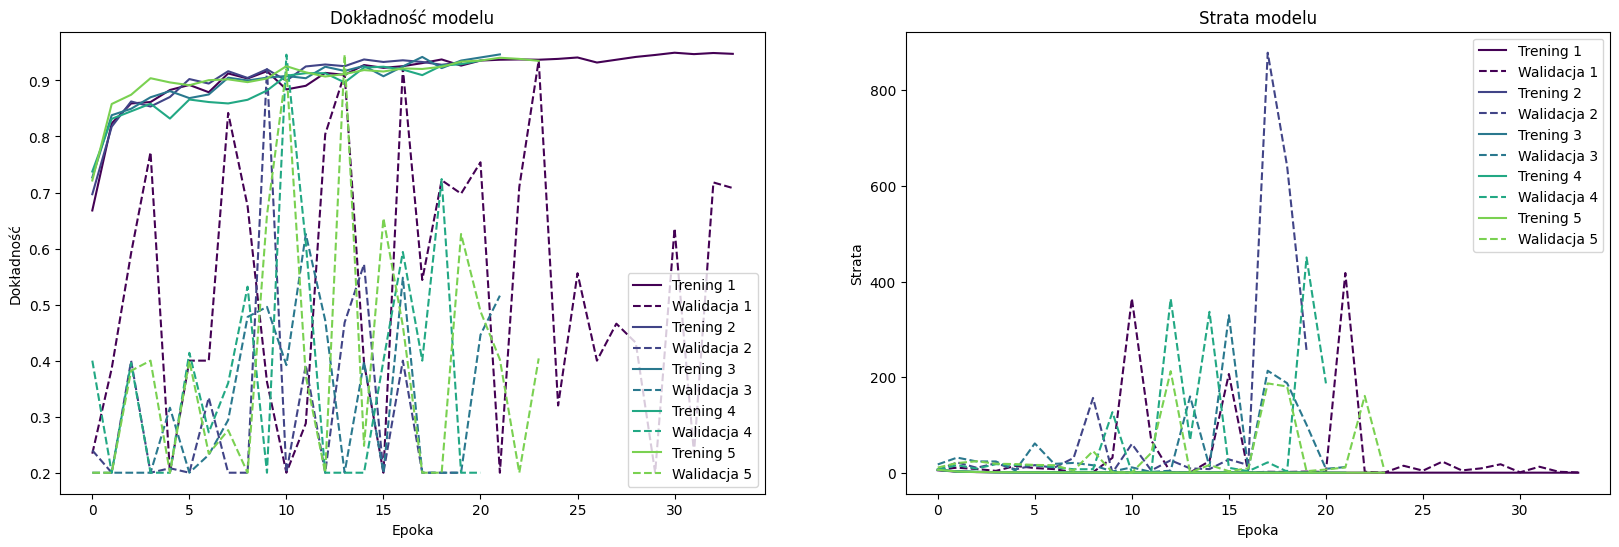
\includegraphics[height=5cm]{resources/tests/images/v4/multiple_edges_crossvalid_img.png}
	\caption{Dokładność i walidacja dla w pełni zmodyfikowanego modelu ze zmienną liczbą wierzchołków i walidacją krzyżową}
	\label{Fig:tests-csvar-2a}
\end{figure}
\FloatBarrier

Model osiąga bardzo wysokie wyniki na zbiorze treningowym,
ale ma problemy z generalizacją na zbiorze walidacyjnym.
Wskazuje to na przeuczenie modelu i brak uczenia się wzorców ogólnych.

\begin{figure}[ht]
	\centering
	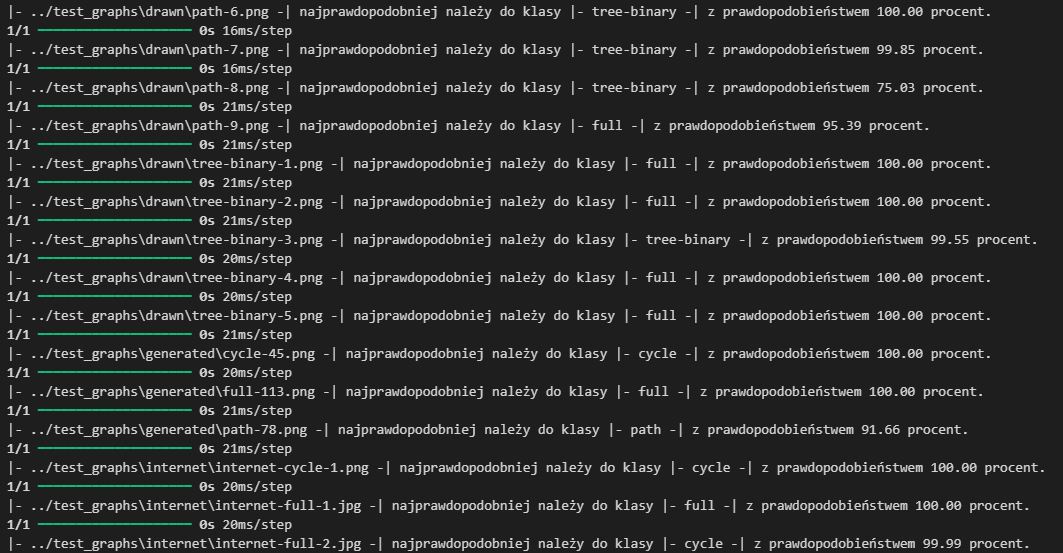
\includegraphics[width=14cm]{resources/tests/images/v4/multiple_edges_crossvalid_txt.png}
	\caption{Klasyfikacja obrazów zewnętrznych dla w pełni zmodyfikowanego modelu ze zmienną liczbą wierzchołków i walidacją krzyżową}
	\label{Fig:tests-csvar-2b}
\end{figure}
\FloatBarrier

\begin{figure}[ht]
	\centering
	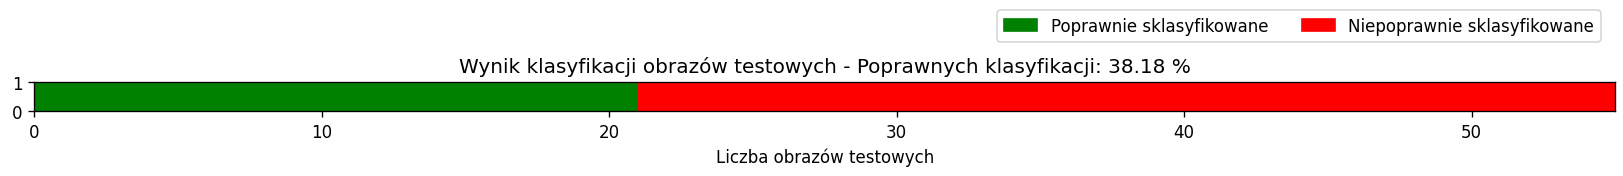
\includegraphics[width=14cm]{resources/tests/images/v4/multiple_edges_crossvalid_bar.png}
	\caption{Wizualizacja klasyfikacji obrazów zewnętrznych dla w pełni zmodyfikowanego modelu ze zmienną liczbą wierzchołków i walidacją krzyżową}
	\label{Fig:tests-csvar-2c}
\end{figure}
\FloatBarrier

Model ocenił poprawnie około 38\% klas grafów zewnętrznych, co nie jest złym wynikiem.
W przypadku modeli z walidacją krzyżową, zastosowanie wszystkich przygotowanych modyfikacji modelu,
nie do końca spełniło swoje złożenia, ale również nie pogorszyło wyniku.